\subsection{BorderGuard Using Indirect iBGP Feeds}
\label{sec:algo}

In this subsection, we describe the algorithm that detects inconsistent
route advertisements from peers, using only data that are directly
available to that AS.
%, such as iBGP routing information and
%its own routing policy.  
We first define this new problem and explain the challenges for
inferring the characteristics of eBGP advertisements from iBGP data
and routing policy.  We state the conditions that must be true in
order for this inference to be possible.  We then present an algorithm
that accurately determines whether a peer advertises consistent
routes at all peering points as long as these conditions are
satisfied.


\paragraph{Problem Formulation}

\begin{figure}
\begin{center}
\begin{psfrags}
\psfrag{b1}{$b_1$}
\psfrag{b2}{$b_2$}
\psfrag{b3}{$b_3$}
\resizebox{0.6\textwidth}{!}{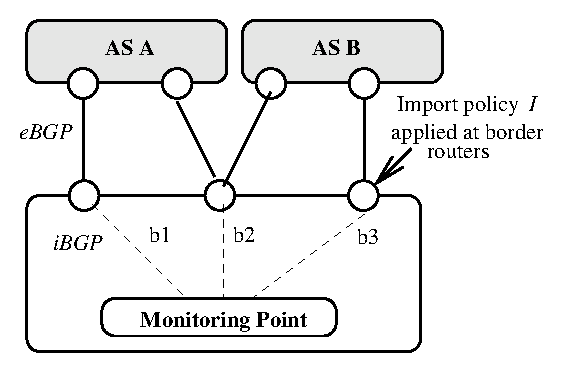
\includegraphics{dynamic/figures/overview.eps}}
\end{psfrags}
\end{center}
%\centering{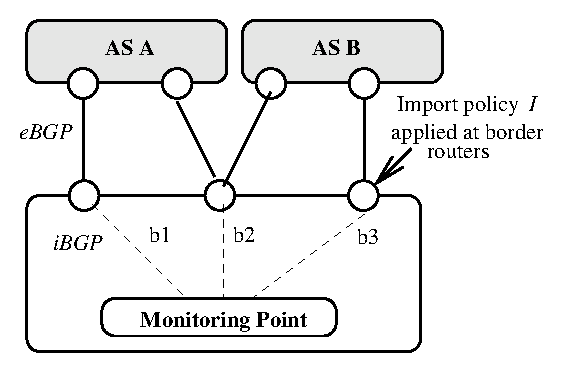
\epsfig{file=dynamic/figures/overview.eps,width=0.5\linewidth}}
\caption[Monitoring inconsistent route advertisements]{Monitoring inconsistent route advertisements in an AS with
  three peering points.}
\label{fig:summary}
\end{figure}

%We now formally define the problem of detecting inconsistent
%eBGP-learned routes using iBGP information and policy data.  
An AS has $k$ border routers, each of which may have zero or more
sessions to each of the AS's peers.  We also define a function
$\mathit{Routers}(p)$ that returns the set of $n_p$ routers in the AS
that peer with $p$.  Each border router $i$ applies an import policy,
$I_i$, to the routes that it receives via eBGP and selects a single
best route $b_i$ for a destination.  In practice, $I$ is actually
configured and applied on a per-session basis, rather than a
per-router basis, but we abstract this detail to simplify
notation. Each router $i$ then distributes the route $b_i$ to other
routers in the AS via iBGP.  An AS can get access to the routes $b_1,
b_2, \ldots, b_k$ using iBGP sessions to a route monitor, as shown in
Figure~\ref{fig:summary}; many ASes already deploy such a monitor.
The values of $\mathit{Routers}(p)$ and $I_i$ are readily available
from the router configuration data.

%% \begin{itemize}
%% %\item $k$ border routers $i = 1, \ldots, k$ 
%% %\item function $Routers(p)$ gives set of $n_p$ routers that peer with $p$
%% \item best route $b_i$ for $i = 1, \ldots, k$ after BGP decision process
%%          in Table~\ref{tab:decision} is applied at router $i$ 
%% \end{itemize}

Access to the only the {\em best\/} routes limits an AS's ability to
directly determine whether a peer advertised a route at some
router (as well as the characteristics of the advertised route): the
alternate routes at the border routers are not available.  To
determine the properties of the complete set of routes that any peer
advertises, we must devise an algorithm that takes the set
of best routes as input and infers properties about the routes
from a peer that are not in that set.

Our inference algorithm applies the following insight: {\em the route
  $b_i$ that router $i$ selects must be at 
least as good as all other routes learned at router $i$, according to
the first five steps of BGP decision process}.  Using this insight, we
can often make the following assertion: if a peer $p$ advertises routes
$r_{p,u}$ and $r_{p,v}$ to two distinct border routers and the
router that learns $r_{p,u}$ selects it as the best route but the router
that learns $r_{p,v}$ selects a route that is {\em worse} than $r_{p,u}$
according to the first five steps of the BGP decision process, then
$\lambda(r_{p,u}) > \lambda(r_{p,v})$ (\ie, peer $p$ advertised
inconsistent routes).
In many cases, we can make assertions about
$\lambda(r_{p,v})$, {\em even though the monitoring point never sees
$r_{p,v}$}, based on the fact that $r_{p,v}$ is missing from the set of
best routes.  In the next subsection, we describe the constraints necessary
to make this determination and also explain the cases where our
algorithm cannot make accurate inferences.

%% or not) -- so, we need to have an inference algorithm that operates on
%% what we did actually see to tell us about what we didn't see...  we do
%% know that no route that was better by the decision process in
%% Table~\ref{tab:decision} was available for selection at router $i$.
%% problem is that this decision incorporates attributes set by the local
%% AS's import policy (\eg, local pref) and the attributes sent by the
%% peer (\eg, AS path length), and we need to pull that apart and see
%% what we can infer about what the peer actually sent.  

\paragraph{Limitations on Inferring Violations}\label{sec:limit}

Access to only the import policies and iBGP routes from border routers
presents several limitations and challenges for inferring 
inconsistent route advertisements.  

{\bf Import policies change route attributes.} 
%The border routers
%  may apply local {\em import policies} before selecting a best route and
%  readvertising it via iBGP.  
Routes that the iBGP monitor sees as inconsistent may in fact be
  caused by the import policy locally at border routers, and routes
  that appear consistent {\em with each other} at the iBGP monitor do
  not ensure that a peer is sending consistent route advertisements.
%  We define $I_i$ as the function that applies the import policy
%  applied to routes learned at router $i$; we can accurately determine
%  the function by examining router configurations.
  The monitor only
  observes $b_i$, but to detect inconsistencies in routes as sent by
  the peer that advertised that route ($peer(b_i)$), we must be able
  to determine the route that the peer actually advertised before
  import policy transformation (\ie, $I_i^{-1}(b_i)$). To ensure
  that, given $b_i$ and $p = peer(b_i)$, the algorithm can determine
  the corresponding $r_{p,u}$ (\ie, the route that the peer initially
  sent), we require the following condition:

\begin{constraint}[Invertible import policy]\label{c:invert}
For all $i \in [1,k]$, $I^{-1}_i$ is computable.  That is, it is
possible to recover the route that $peer(b_i)$ initially advertised by
applying $I^{-1}_{i}(b_i)$.
\end{constraint}

Import policies often overwrite certain route attributes (\eg, MED) on
routes learned from peers, unless the AS has agreed in advance to accept
them.  Overwriting a route attribute is not invertible, so this
operation violates Condition~\ref{c:invert}.  Fortunately, the inability
to determine these route attributes does not matter in a practical
setting, because the AS can {\em force\/} these attributes to be
consistent by overwriting the attributes in the same way (\eg, a common
practice is to set MED values to $0$ on all routes learned from a peer).
The inference algorithm is most useful when a peer is sending
inconsistent routes {\em in a way that import policy cannot rectify}
(\eg, inconsistent AS path lengths or missing route advertisements).

%\footnote{Import policies that perform AS path
%prepending on inbound eBGP-learned routes are almost always
%invertible.  A rare exception is the case where an AS might prepend
%the peer's AS number $n$ times upon hearing a route of length $l$ and
%$n+m$ times upon hearing a route of length $l-m$: in both cases, the
%resulting AS path would be of length $l+n$, but a router that learned
%this route via iBGP would not be able to determine whether the
%original AS path was of length $l$ or $l-m$.}  



{\bf Import policy can make consistent routes appear
   inconsistent.}  The algorithm must infer
   properties of a route that it might not see.  Because we are
   interested in determining the properties of such a route {\em before}
   a router applies import policy, we must assume that the import policy
   {\em at a single router} treats all routes $r$ for which $\lambda(r)$ is
   equal in exactly the same way.  That is, the import policy at each
   router should not treat two routes that are consistent in a way that
   would make them inconsistent. 

\begin{constraint}[Consistent treatment of consistent
   routes.]\label{c:consistent} 
If $\lambda(r_{p,i})=\lambda(r_{p,j})$ then 
  $\lambda(I_{i}(r_{p,i}))=\lambda(I_{i}(r_{p,j}))$.
\end{constraint}

The inference algorithm should be able to infer how route $r_{p,j}$would
have been treated by our import policy at $i$ if that route were
``consistent'' with $r_{p,i}$.  Otherwise, it is impossible to tell
whether the AS's import policy caused the consistency violation or
whether the inconsistency was caused by a peer.

\begin{figure}
\begin{center}
\begin{psfrags}
\psfrag{b1}{$b_1$}
\psfrag{b2}{$b_2$}
\psfrag{b3}{$b_3$}
%{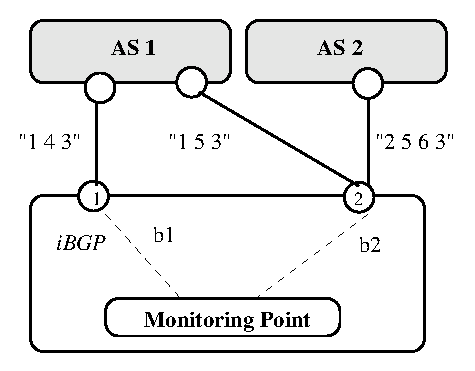
\epsfig{file=dynamic/figures/ambiguity.eps,width=0.5\linewidth}}
\resizebox{0.5\textwidth}{!}{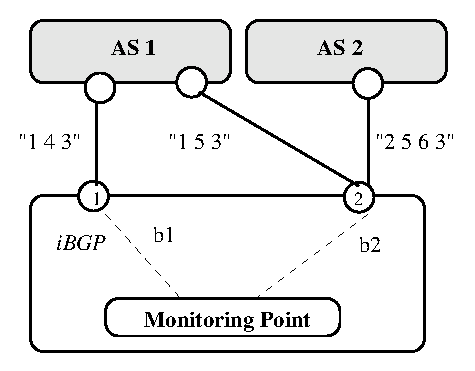
\includegraphics{dynamic/figures/ambiguity.eps}}
\end{psfrags}
\end{center}
\caption{Example illustrating different AS paths (with the same AS path
  {\em length}) from the same peer.}
\label{fig:ambig}
\end{figure}


Figure~\ref{fig:ambig} explains how a violation of this constraint can
cause ambiguity.  In this case, the AS's peer $p$ advertises a route
$r_{p,1}$ with AS path ``1 4 3'' at one border router and a route
$r_{p,2}$ with AS path ``1 5 3'' at a second border router; assume that
all other route attributes are the same.  Note that these routes are
{\em consistent}: $\lambda(r_{p,1})=\lambda(r_{p,2})$, because the AS
path {\em lengths} are the same.  If router $2$ applied a policy that,
for example, assigned a lower local preference to routes with AS path
``1 5 3'', then router $1$ could conceivably select a route $r_{q,1}$ from
another peer $q$.
We would like to be able to say that $\lambda(r_{p,1})$ must be worse
than $\lambda(r_{p,2})$ (\ie, that the routes are inconsistent), but we
cannot do so: it is impossible to distinguish between the case where
$p$ sends route ``1 5 3'' and router $1$ selects a route from $q$ and
the case where $p$ sends a route with a longer path length to router $1$
(or does not send any route).

Unfortunately, this constraint is occasionally violated.  For these
peers and sessions, we cannot detect inconsistent
advertisements from iBGP messages alone. Nevertheless, we were still
able to perform our analysis on the vast majority of peers; we discuss
our analysis further in Section~\ref{sec:results}.

{\bf Inability to distinguish inconsistent routes from a missing route.}
Because it has direct access to eBGP messages, the algorithm in
Section~\ref{sec:problem} is able to distinguish between two separate
cases of inconsistent advertisements: (1)~when a peer sends routes with
inconsistent attributes to one or more peering points and (2)~when a
peer fails to send {\em any} route for a prefix to one or more peering points.
With access to only the best routes from each router, however, the
inference algorithm cannot determine whether a border router did not select
a route from peer $p$ because the route from $p$ looked ``worse'' than
other routes learned at that router or because $p$ did not advertise any
route at all to that router.  Because the {\em effect} of either of
these inconsistencies is the same---in either case, the AS may be forced
to do ``cold potato'' routing---it is not crucial that the inference
algorithm be able to distinguish between these two cases.


{\bf Arbitrary path selection tiebreaking.}  The BGP decision process
may break ties between two routes $r_1$ and $r_2$ for which
$\lambda(r_1)=\lambda(r_2)$ arbitrarily (\eg, based on the router ID
of the router from which the route was learned or on which route was
learned first).  As a result, the inference algorithm may not be able
to detect whether a given peer $p$ advertised consistent routes to a
destination if $\lambda(b_i)=\lambda(b_j)$ but $b_i$ and $b_j$ are
learned from two different peers, $p$ and $q$.  For example, suppose
that $\lambda(r_{p,u})=\lambda(r_{q,u}) =\lambda(r_{p,v})$, but the
tiebreaking stage at router $i$ selects the route from peer $q$.  In
this case, the inference algorithm cannot determine whether the routes
advertised by $p$ are consistent, because $\lambda(b_i)=\lambda(b_j)$:
the route from router $i$ is not strictly worse, so a consistent
$r_{p,i}$ could have existed, but it is impossible for the AS to
invert this based on $b_i$ and $b_j$ alone.

Arbitrary tiebreaking of equally-good eBGP-learned routes at a given
border router may occur frequently\footnote{It is not uncommon for
routes to the same destination from multiple peers to be ``equally
good'' in terms of local preference, AS path length, MED, and origin
type.  For example, an enterprise might multihome to two or more of an AS's
peers; both peers will advertise routes to that customer with the same
path length.  In these cases, border routers will break ties
arbitrarily.} and it prevents the inference algorithm from determining
whether a peer advertised a consistent route to that router.
Fortunately, this scenario can only arise if one peer 
advertises a route to that router {\em that is equally good as the other
peer's advertisements}.  If tiebreaking prevents inference at a given router,
another equally good route must exist at that router, and ``cold
potato'' routing will not occur anyhow: the routers in the AS that would
have chosen a consistent route from that peer at that router will
instead use the alternate route (rather than sending traffic to another
border router), since the route they learn from that peering is as good
as the consistent route would have been.





%% \begin{itemize}
%% %\item $I_i$ import policy at router $i$ (from config)
%% \item function $peer(b_i)$ gives peer (next-hop) associated with route $b_i$
%%          (from the routes themselves)
%% \end{itemize}

%\begin{itemize}
%% \item invertible import policy: \ie, from $I_i$ we can get $I^{-1}_i$
%%         to go from $b_i$ to $I^{-1}_{i}(b_i)$ (so we can learn what 
%%         route our peer initially sent to us at router $i$
%\end{itemize}

\paragraph{BorderGuard Consistency Assertion}

Given the two constraints from the previous subsection and access to both
the iBGP feeds from the border routers, ($b_1 \ldots b_k$), and the import
policies, ($I_1 \ldots I_k$), an AS can now determine whether its peer $p$ is
sending inconsistent advertisements at different peering points by
testing the following assertion:

\vspace{0.05in}
\begin{center}
\begin{tabular}{|l|}
\hline
for each border router $i$ \hspace*{0.15in} ($i = 1\ldots k$) \\
\hspace*{0.2in} for each router $j\in Routers(peer(b_i))$ \\
\hspace*{0.4in}    $\lambda(b_j) \geq \lambda(I_j(I^{-1}_i(b_i)))$ \\
\hline
\end{tabular}
\end{center}
\vspace{0.05in}

\begin{figure}
\begin{center}
\begin{psfrags}
\psfrag{mp}{$p$}
\psfrag{bi}{$b_i$}
\psfrag{bj}{$b_j$}
\psfrag{rpv}{$r_{p,v}$}
\psfrag{rpu}{$r_{p,u} = I_i^{-1}(b_i)$}
%{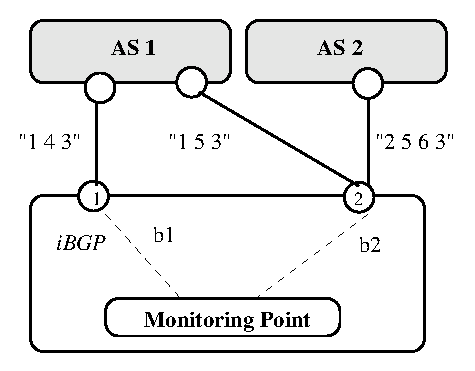
\epsfig{file=dynamic/figures/ambiguity.eps,width=0.5\linewidth}}
\resizebox{0.5\textwidth}{!}{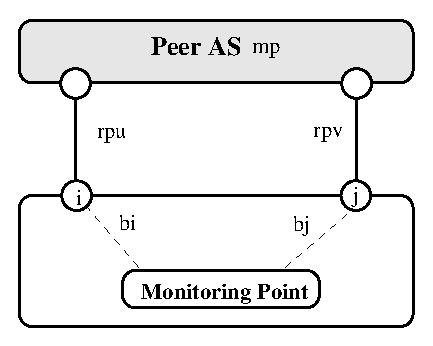
\includegraphics{dynamic/figures/invariant.eps}}
\end{psfrags}
\end{center}
\caption{Applying the BorderGuard consistency assertion}
\label{fig:invariant}
\end{figure}


If this condition is violated, then peer $p=peer(b_i)$ has failed to send a
consistent advertisement to router $j$.  Figure~\ref{fig:invariant}
explains the intuition behind this result.  Ultimately, for each router
$i$ that selects a best route $r_{p,u}$, the AS must
verify the following condition on routes learned from peer $p$:
\vspace{-0.05in}
\begin{eqnarray*}
\lambda(r_{p,u}) & = & \lambda(r_{p,v}) 
\end{eqnarray*}
given only $b_i$ and $b_j$.  We can compute $r_{p,j}$ using
Constraint~\ref{c:invert} 
to invert the import policy at router $i$ on $b_i$:
\begin{eqnarray*}
\lambda(I^{-1}_u(b_i)) & = & \lambda(r_{p,v}) 
\end{eqnarray*}
Finally, we can apply Condition~\ref{c:consistent} to obtain:
\begin{eqnarray*}
\lambda(I_j(I^{-1}_i(b_i))) & = & \lambda(I_j(r_{p,v})) 
\end{eqnarray*}
\noindent
This condition must be true if $peer(b_i)$ is sending consistent
advertisements (\ie, $\lambda(r_{p,u}) = \lambda(r_{p,v})$), based on
our observation of $b_u$, {\em even through the monitoring point may not
observe $I_j(r_{p,v})$}.  If the monitoring point receives a $b_j$ such
that $\lambda(b_j)$ is strictly less than $\lambda(I_j(I^{-1}_i(b_i)))$
(\ie, the ranking of a consistent route from $peer(b_i)$ after router
$j$ applies import policy), then $\lambda(r_{p,u}) \neq
\lambda(r_{p,v})$. That is, either peer $p$ did not advertise a route to
router $j$, or the attributes $r_{p,v}$ were strictly worse than those
of $r_{p,u}$.

Testing this assertion in a live network is straightforward.  Both the
set of $k$ border routers and the set of routers that peer with a peer
$p$, $Routers(p)$, are readily available from the router configuration.
$I_j$ and $I_i^{-1}$ can also be determined from the import policies
defined in the router configurations. $peer(b)$ for any best route is
also easy to compute: it is simply the first AS in the AS path
attribute of the route.  Starting with a table dump of the routes, the
monitor can directly test the assertion for every $b_i$ for all prefixes;
in steady state, detection is more
lightweight: whenever any best route $b_i$ changes, the algorithm can
simply test the assertion for that best route, rather than re-executing
the check for all ($b_1 \ldots b_k$).
%% Finally, we note that this
%% algorithm need not be centralized: each border router $j$ in the AS has
%% all information that is necessary for testing the assertion locally
%% available, with the exception of $I_i^{-1}(b_i)$, which router $i$ could
%% forward to router $j$ via a special monitoring session.

%note that we apply the converse of constraint 2 to identify cases
%where $\lambda(r_{p,i})\neq\lambda(r_{p,j})$.
